\section{Symmetry of the gems}
\label{sec:symmetry}

Let $\rho(x,y,z)=(x,y,-z)$ be the reflection in the plane $z=0$.
The \emph{complement} of an arrangement is $\overline S=N+1-S$ (so $\overline S$ has height function $-z$), and $S$ is \emph{associative} if $S+r^2S=N+1$, where $r^2$ is the half-turn of the grid; $S$ is \emph{self-complementary} if $\overline S=gS$ for some $g\in D_4$.
Complements of magic squares are magic.

\begin{lemma}[Complement is a mirror image]
\label{lem:complement}
$\mathcal G(\overline S)=\rho\,\mathcal G(S)$.
If $\overline S=gS$ with $g\in D_4$, then $\iota_g:=\hat g^{-1}\rho$, i.e.\ $\iota_g(x,y,z)=(g^{-1}(x,y),-z)$, is an isometry of $\R^3$ mapping $\mathcal G(S)$ onto itself, with $\det\iota_g=-\det g$.
\end{lemma}

\begin{proof}
The points of $\overline S$ are $(x_c,y_c,-z_c)=\rho\,\mathbf p_c$. If $\overline S=gS$ then $\rho\,\mathcal G(S)=\mathcal G(\overline S)=\mathcal G(gS)=\hat g\,\mathcal G(S)$ by \Cref{prop:symmetry_invariance}, so $\hat g^{-1}\rho\,\mathcal G(S)=\mathcal G(S)$.
\end{proof}

\begin{proposition}[Which elements of $D_4$ can complement]
\label{prop:selfcomp}
Let $\overline S=gS$ for an arrangement $S$ of order $n\ge2$. Then $g^2=\mathrm{id}$ and $g$ has no fixed cell other than possibly the centre cell of an odd grid, whose entry is then $(N+1)/2$.
Consequently:
\begin{enumerate}
\item for $n$ odd, $g=r^2$, so $S$ is associative;
\item for $n$ even, $g\in\{r^2,h,v\}$ with $h,v$ the left--right and top--bottom reflections; the diagonal reflections and the quarter-turns never occur.
\end{enumerate}
The corresponding isometries of $\mathcal G(S)$ are $\iota_{r^2}(\mathbf p)=-\mathbf p$ (point reflection, improper), $\iota_h(x,y,z)=(-x,y,-z)$ (half-turn about the $y$-axis, proper) and $\iota_v(x,y,z)=(x,-y,-z)$ (half-turn about the $x$-axis, proper).
\end{proposition}

\begin{proof}
Applying $g$ to $\overline S=gS$ gives $g\overline S=\overline{gS}=S$, so $g^2S=\overline{\overline S}=S$; since the entries are distinct, $g^2$ fixes every cell, hence $g^2=\mathrm{id}$ ($D_4$ acts faithfully on the cells for $n\ge2$).
If $g$ fixes a cell $c$ then $s_c=N+1-s_c$.
The involutions of $D_4$ are $r^2$, $h$, $v$ and the two diagonal reflections.
The diagonal reflections fix $n\ge2$ cells and are excluded; $h$ and $v$ fix the $n$ cells of the middle column (row) when $n$ is odd, and none when $n$ is even; $r^2$ fixes only the centre cell when $n$ is odd.
For $n$ odd the centre cell is the only cell that can have the value $(N+1)/2$, so $g=r^2$.
The formulas for $\iota_g$ follow from \Cref{lem:complement}, and the determinants are $-\det r^2=-1$, $-\det h=-\det v=+1$.
\end{proof}

By \Cref{prop:selfcomp}, associative squares give gems with a point reflection: \emph{centrally symmetric} gems.
(Every Siamese square is associative, which explains the symmetric vertex list in \Cref{prop:siamese-12}; D\"urer's square is associative and its gem is centrally symmetric, \Cref{fig:symmetry}a, \Cref{fig:pointsets}a.)
Self-complementary squares that are not associative give gems with a half-turn symmetry.
For order four we determine the complete isometry group of every gem.
For a finite set $X\subset\R^3$ let $\operatorname{Iso}(X)$ be the group of isometries of $\R^3$ mapping $X$ to itself.

\begin{theorem}[Isometry groups of the order-four gems; computer-assisted]
\label{thm:symmetry}
Let $S$ be one of the $880$ essentially different magic squares of order $4$ and $\mathcal G=\mathcal G(S)$. Then $\operatorname{Iso}(\mathcal G)=\operatorname{Iso}(V)=\operatorname{Iso}(\{\mathbf p_{ij}\})$, where $V$ is the vertex set, and:
\begin{enumerate}
\item $S$ is associative ($48$ squares, Dudeney's group III) if and only if $\operatorname{Iso}(\mathcal G)=\{\mathrm{id},-\mathrm{id}\}$ (the group $C_i$);
\item $S$ is self-complementary but not associative ($304$ squares, Dudeney's group VI) if and only if $\operatorname{Iso}(\mathcal G)=\{\mathrm{id},\iota\}$ with $\iota$ a half-turn about a horizontal coordinate axis (the group $C_2$);
\item for the remaining $528$ squares $\operatorname{Iso}(\mathcal G)$ is trivial.
\end{enumerate}
Consequently $\mathcal G(S)$ has an improper isometry if and only if $S$ is associative; the $832$ gems of the cases (2) and (3) are chiral; and the congruence classes of the $880$ gems number $48+304+264=616$, the $528$ gems of case (3) forming $264$ pairs $\{\mathcal G(S),\mathcal G(\overline S)\}$ of mirror images in the plane $z=0$.
\end{theorem}

\begin{proof}
The inclusions ``$\supseteq$'' and the identification of the generators for the associative and self-complementary squares are \Cref{lem:complement} and \Cref{prop:selfcomp}; the classes (1), (2) are exactly the self-complementary ones, which were counted as $48$ and $304$ (all of the form $h$ or $v$ after \Cref{prop:selfcomp}) by exact comparison of the $8$ images of $S$ with $\overline S$.
For the reverse inclusions we computed, for each of the $880$ squares, \emph{all} isometries of its vertex set and of its $16$-point set, in exact integer arithmetic: the vertex set is centred at its centroid (scaled to integers), the images of three linearly independent vertices are enumerated among the vertices with the same Gram matrix entries, each candidate orthogonal map is accepted only if the induced bijection of the vertices preserves all pairwise integer squared distances (\Cref{sec:appendix}).
This yields the group orders $2,2,1$ in the three cases, equal for the vertex set and the $16$-point set; since $\mathcal G$ is the convex hull of $V$, $\operatorname{Iso}(\mathcal G)=\operatorname{Iso}(V)$ (an isometry preserves extreme points).
A gem is chiral if it has no improper isometry; the group $C_2$ consists of proper maps, which gives the chirality statement.
Finally, congruent gems come from the same complement orbit (\Cref{prop:gem-injective}), and in case (3) the classes of $S$ and $\overline S$ are distinct, giving $264$ pairs.
\end{proof}

\begin{table}[htbp]
\centering
\caption{Symmetry types of the $880$ order-four gems. $V$: number of hull vertices; ``classes'' counts congruence classes of gems.}
\label{tab:symmetry}
\small
\begin{tabular}{p{3.6cm} c r p{2.6cm} r l}
\toprule
type of $S$ & Dudeney & squares & $\operatorname{Iso}(\mathcal G)$ (order) & classes & $V$\\
\midrule
associative & III & $48$ & $C_i$, inversion ($2$) & $48$ & $10,12,14,16$\\
self-complementary, not associative & VI & $304$ & $C_2$, half-turn ($2$) & $304$ & $8,10,12,14,16$\\
neither & others & $528$ & trivial ($1$) & $264$ & $8,\dots,16$\\
\midrule
total & & $880$ & & $616$ &\\
\bottomrule
\end{tabular}
\end{table}

\begin{proposition}[Facet orbits]
\label{prop:facet-orbits}
Let $S$ be one of the $880$ squares and let $\operatorname{Iso}(\mathcal G)$ act on the facets of $\mathcal G$.
\begin{enumerate}
\item If $S$ is associative, every facet $F$ has a distinct antipodal partner $-F$, a facet in the parallel plane on the other side of the origin; so there are no fixed facets and the facets form $F/2$ antipodal pairs. Here $F\in\{12,14,16,18,20,22\}$ with $1,12,12,17,4,2$ gems respectively, and $V\in\{10,12,14,16\}$ with $13,28,4,3$ gems. The partner $-F$ has the opposite outward normal; as plane polygons $F$ and $-F$ are congruent by a rotation through $\pi$, although the point reflection carrying $F$ to $-F$ is improper.
\item If $S$ is self-complementary and not associative, with half-turn $\iota$ about the $y$-axis (say), the facet orbits have size $1$ or $2$. A facet is fixed if and only if it lies in $y=\pm\frac32$; such a facet is a parallelogram (the hull of the top or bottom row), and exists unless the four points of that row are collinear. There are two fixed facets for $282$ gems, one for $18$ and none for $4$.
\item The vertices of a gem with a symmetry fall into orbits of size $2$, so $V$ is even for the $352$ self-complementary squares.
\end{enumerate}
\end{proposition}

\begin{proof}
Both nontrivial isometries fix the origin, which is an interior point of $\mathcal G$ (\Cref{prop:centroid}), so no facet plane $\{\mathbf n\cdot\mathbf p=d\}$ has $d=0$.
(1) $-F\neq F$ because $-$ maps the facet plane $\mathbf n\cdot\mathbf p=d$ to $\mathbf n\cdot\mathbf p=-d\ne d$.
(2) The half-turn $\iota=(x,y,z)\mapsto(-x,y,-z)$ maps the plane $\mathbf n\cdot\mathbf p=d$ to $\iota\mathbf n\cdot\mathbf p=d$, which is the same plane iff $\iota\mathbf n=\mathbf n$, i.e.\ $\mathbf n\parallel(0,1,0)$; the facet planes with this normal are $y=\pm\frac32$.
The hull of the top row (the points with $y=\frac32$) is $\iota$-invariant; its vertices come in pairs $\pm(x,z)$ and a convex polygon with at most four vertices and a centre of symmetry is a segment or a parallelogram.
The counts are those of the exact computation.
(3) $\iota$ and $-\mathrm{id}$ fix no vertex: the half-turn fixes only points with $x=z=0$, while $x$ is a half-odd integer; the point reflection fixes only the origin.
\end{proof}

\begin{proposition}[Parity of the point types for associative squares]
\label{prop:parity}
Let $S$ be associative of order $n$ and let $V,I,B$ be the numbers of vertices, strictly interior points and boundary non-vertex points of $\mathcal G(S)$.
Then $V$ and $B$ are even, and $I\equiv n\pmod 2$.
In particular for even $n$ all three numbers are even.
\end{proposition}

\begin{proof}
Associativity says that the cell $c'$ opposite to $c$ carries $s_{c'}=N+1-s_c$, so $\mathbf p_{c'}=-\mathbf p_c$: the point set is invariant under the linear isometry $-\mathrm{id}$, which therefore maps $\mathcal G(S)$ to itself, and permutes its vertices, its strictly interior points and its boundary non-vertex points among themselves.
The only fixed point of $-\mathrm{id}$ is the origin, which is a point $\mathbf p_{ij}$ only if $n$ is odd (the central cell has $s=\frac{N+1}2$), and then it is strictly interior by \Cref{prop:centroid}.
Hence the involution is fixed-point free on vertices and on boundary non-vertex points, and on strictly interior points when $n$ is even; for odd $n$ it fixes exactly one of the latter.
\end{proof}

For $n=4$ the $48$ associative gems have $V\in\{10,12,14,16\}$ and $I\in\{0,2,4\}$ ($4$, $23$ and $21$ gems), in accordance with \Cref{prop:parity} (exact computation, \texttt{anc/box\_and\_classes.py}); among the non-associative squares both parities of $I$ occur.

\begin{figure}[htbp]
\centering
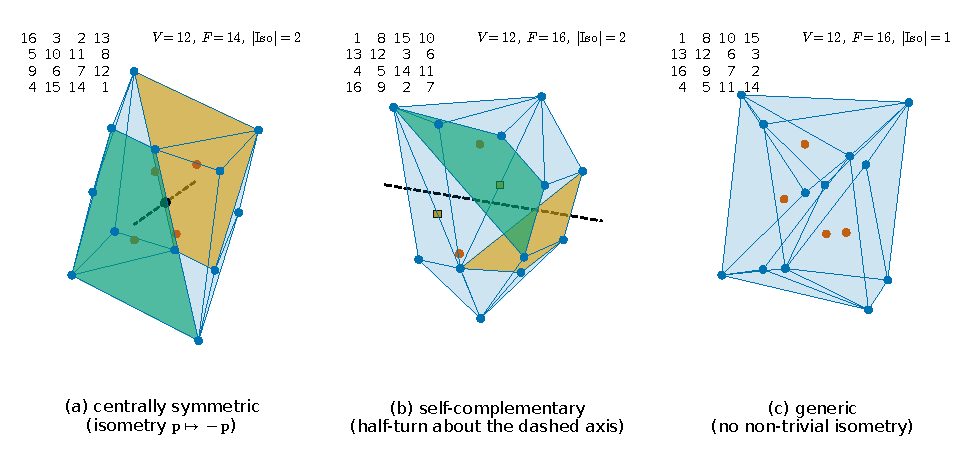
\includegraphics[width=\textwidth]{figures/fig_symmetry.pdf}
\caption{Symmetry types of order-four gems (same viewpoint; strictly interior points are red discs, boundary non-vertex points orange squares; the square is printed above each gem).
(a)~D\"urer's square: a centrally symmetric gem; an antipodal pair of facets $F$ (orange) and $-F$ (green) and the segment joining their centroids through the centre $\mathbf 0$ (dashed).
(b)~A self-complementary, non-associative square (square \#124): the half-turn $\iota$ about the dashed axis swaps the highlighted pair of facets and has no other symmetry.
(c)~A square with no symmetry (square \#102): the gem is chiral, and its mirror image in $z=0$ is the gem of the complement $17-S$.}
\label{fig:symmetry}
\end{figure}

\Cref{fig:pointsets} shows the same three squares as point sets in the height picture: for the associative square the $16$ points form $8$ antipodal pairs $\{\mathbf p,-\mathbf p\}$ whose segments all pass through $O$; for the self-complementary square the half-turn about the dashed horizontal axis exchanges the $8$ pairs, each segment meeting the axis perpendicularly at its midpoint; the third square has no such pairing, in agreement with \Cref{thm:symmetry}.

\begin{figure}[htbp]
\centering
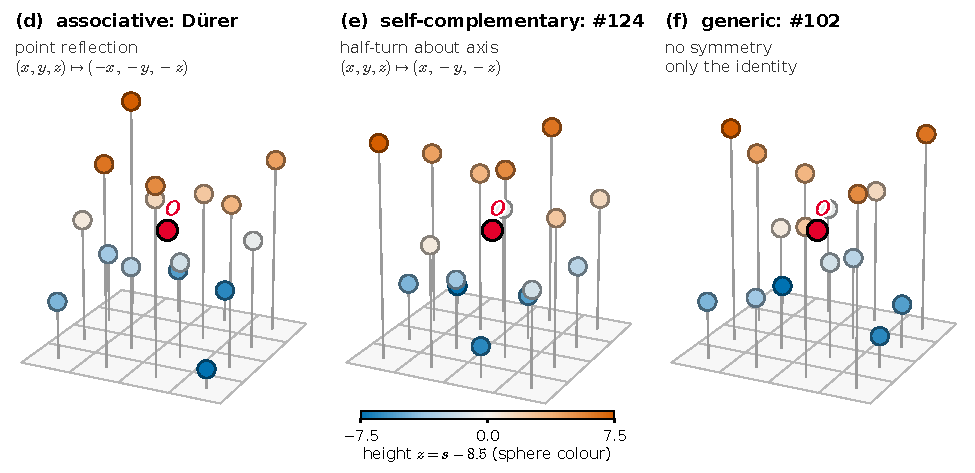
\includegraphics[width=\textwidth]{figures/fig_pointsets.pdf}
\caption{The $16$ points $\mathbf p_{ij}$ as spheres on stems over the floor grid, coloured by height $z$ (same squares and viewpoint as \Cref{fig:symmetry}; $O$ red). (a)~D\"urer's square: the points form $8$ antipodal pairs $\{\mathbf p,-\mathbf p\}$, joined by segments through $O$. (b)~Square \#124: the half-turn $(x,y,z)\mapsto(x,-y,-z)$ about the dashed $x$-axis exchanges $8$ pairs of points, each pair joined by a segment perpendicular to the axis; this gem is chiral. (c)~Square \#102: no non-trivial isometry preserves the point set.}
\label{fig:pointsets}
\end{figure}

\begin{remark}[Classes of order-four squares and vertex counts; exact computation]
\label{rem:classes}
Dudeney's group I consists exactly of the $48$ pandiagonal squares (all broken diagonals sum to $34$), group III of the $48$ associative squares, and group VI of the $304$ self-complementary non-associative squares, whose gems have the half-turn symmetry of \Cref{thm:symmetry}; no order-four square is both pandiagonal and associative.
The gems of the $48$ pandiagonal squares have $11$ to $15$ vertices ($10,20,12,4,2$ gems with $11,\dots,15$), never $16$ and never at most $10$, and each has between one and four strictly interior points.
The $7$ gems with $8$ vertices are squares \#50, \#54, \#672 (group VI) and \#276, \#277, \#494, \#496 (group VIII); none is pandiagonal or associative, and each has $I=B=4$.
\end{remark}

\begin{remark}[Central-symmetry defect]
\label{rem:sigma}
For a convex body $K\subset\R^3$ let $\sigma(K)=\operatorname{vol}\bigl(\tfrac12(K-K)\bigr)/\operatorname{vol}(K)$.
The Brunn--Minkowski inequality gives $\operatorname{vol}(K-K)^{1/3}\ge\operatorname{vol}(K)^{1/3}+\operatorname{vol}(-K)^{1/3}=2\operatorname{vol}(K)^{1/3}$, that is $\sigma(K)\ge1$, and for bodies with non-empty interior equality holds if and only if $K$ and $-K$ are homothetic \cite{schneider2014convex}; since they have equal volume the homothety is a translation, so $\sigma(K)=1$ if and only if $K$ is centrally symmetric.
The defect $\sigma$ is invariant under all isometries including reflections, so $\sigma(\mathcal G(S))=\sigma(\mathcal G(\overline S))$ and $\sigma$ is constant on $D_4$-orbits.
For the $880$ order-four gems, $\sigma$ was computed in exact rational arithmetic from the convex hull of the $256$ pairwise differences of the points (\texttt{anc/central\_symmetry\_defect.py}): $\sigma=1$ for exactly the $48$ associative gems, and $\sigma\in[1057/1018,\,145/88]\approx[1.038,\,1.648]$ for the other $832$, the extremes occurring for squares \#569 and \#218.
\end{remark}
